% =====================================================================
% Springer Nature (sn-jnl) template conversion
% Paper: Kelvin Mode Suppression in Atomic Orbitals: A Vortex-Filament Gap
% Author: Omar Iskandarani
% Date (source): 2025-12-14
% Affiliation: Independent Researcher, Groningen, The Netherlands
% License: © 2025 Omar Iskandarani. All rights reserved.
% DOI: 10.5281/zenodo.18018084
% =====================================================================

% =========================
% 1) Document class choice
% =========================
% \documentclass[referee,pdflatex,sn-mathphys-num]{sn-jnl} % double-spacing option for review
\documentclass[pdflatex,sn-mathphys-num]{sn-jnl}

% =========================
% 2) Core packages (lean)
% =========================
\usepackage[T1]{fontenc}
\usepackage[utf8]{inputenc}
\usepackage{lmodern}
\usepackage{microtype}
\usepackage{graphicx}
\usepackage{booktabs}
\usepackage{amsmath,amssymb,amsfonts}
\usepackage{bm}
\usepackage{siunitx}
% \usepackage{physics}

% TikZ/PGFPlots (used by your figures)
\usepackage{tikz}
\usepackage{pgfplots}
\usepackage{pgfplotstable}
\usepackage{caption}
\pgfplotsset{compat=newest}

% Didactic recap environment (unstyled, minimal)
\usepackage{amsthm}
\theoremstyle{remark}
\newtheorem*{didactic}{Didactic recap}

% ====================================
% 3) Paper metadata macros (edit here)
% ====================================
\newcommand{\papertitle}{Kelvin Mode Suppression in Atomic Orbitals:\\ A Vortex-Filament Gap}
\newcommand{\papershorttitle}{Kelvin-Mode Suppression in Orbitals}
\newcommand{\paperdoi}{10.5281/zenodo.18018084}
\newcommand{\paperorcid}{0009-0006-1686-3961}
\newcommand{\paperemail}{info@omariskandarani.com}
\newcommand{\papercity}{Groningen}
\newcommand{\papercountry}{The Netherlands}
\newcommand{\paperkeywords}{Kelvin modes, vortex filaments, hydrodynamic models, atomic spectroscopy, excitation gap}

% (Optional: legacy swirl macros retained but unused prior to Outlook)
\newcommand{\swirlarrow}{\mkern-2mu\scriptscriptstyle\boldsymbol{\circlearrowleft}}
\newcommand{\vswirl}{\mathbf{v}_{\mkern-2mu\scriptscriptstyle\boldsymbol{\circlearrowleft}}}
\newcommand{\SwirlClock}{S_{(t)}^{\mkern-2mu\scriptscriptstyle\boldsymbol{\circlearrowleft}}}
\newcommand{\Fmaxswirl}{F^{\max}_{\mkern-1mu\scriptscriptstyle\boldsymbol{\circlearrowleft}}}
\newcommand{\Fmax}{F^{\max}_{\mkern-1mu\scriptscriptstyle\boldsymbol{\circlearrowleft}}}
\newcommand{\FmaxEM}{F^{\max}_{\mathrm{EM}}}
\newcommand{\FmaxG}{F_{\mathrm{G}}^{\max}}
\newcommand{\vscore}{v_{\swirlarrow}}
\newcommand{\vnorm}{\lVert \mathbf{v}_{\mkern-2mu\scriptscriptstyle\boldsymbol{\circlearrowleft}} \rVert}
\newcommand{\rhoF}{\rho_{\!f}}\newcommand{\rhof}{\rho_{\!f}}
\newcommand{\rhoE}{\rho_{\!E}}\newcommand{\rhoe}{\rho_{\!E}}
\newcommand{\rhoM}{\rho_{\!m}}\newcommand{\rhom}{\rho_{\!m}}
\newcommand{\omegas}{\boldsymbol{\omega}_{\swirlarrow}}
\newcommand{\Om}{\Omega_{\swirlarrow}}
\newcommand{\rc}{r_c}

\raggedbottom

\begin{document}

% =========================
% 5) Title + author block
% =========================
    \title[\papershorttitle]{\papertitle}

    \author*[1]{\fnm{Omar} \sur{Iskandarani}}\email{\paperemail}
    \affil*[1]{\orgname{Independent Researcher}, \orgaddress{\city{\papercity}, \country{\papercountry}}}

% =========================
% 6) Abstract + keywords
% =========================
    \abstract{%
        In hydrodynamic models where electrons are represented by closed vortex filaments in an incompressible medium, atomic orbitals arise as equilibrium configurations. A key consistency issue is whether internal Kelvin-wave excitations could add thermodynamic corrections large enough to destabilize the hydrogenic spectrum. We show that, absent additional structure, such corrections would exceed spectroscopic bounds by many orders of magnitude. A topological excitation gap in the Kelvin spectrum—of order $\mathcal{O}(10^2\text{--}10^3\,\mathrm{eV})$—naturally suppresses these effects. In this regime, the Schr\"odinger equation functions as a low-energy equation of state, while Kelvin dynamics are inert except under extreme acceleration or high-energy conditions. This separation of scales resolves a central constraint on vortex-filament descriptions of atomic structure.%
    }

    \keywords{\paperkeywords}

    \maketitle

% Global dimensionless temperature ratio
    \newcommand{\epsilonK}{\varepsilon_K} % Dimensionless temperature ratio

% ============================================================
    \section{Introduction}\label{sec:intro}
        Hydrodynamic and vortex-based models of matter trace back to Kelvin and Helmholtz \cite{Helmholtz1858,Kelvin1867}. Modern superfluid dynamics and quantum turbulence have renewed interest in vortex filaments as fundamental excitations \cite{Onsager1949,Feynman1955,Barenghi2014}.

        We consider a conservative vortex-filament picture in which closed, knotted filaments embedded in an incompressible medium encode electron degrees of freedom. Prior work indicates that the hydrogenic spectrum can follow from hydrodynamic force balance, with the Schr\"odinger equation emerging as the Euler–Lagrange condition of an appropriate free-energy functional.

        A natural objection is the presence of \emph{Kelvin waves}—helical filament excitations \cite{LordKelvin1880,Barenghi2014}. If these modes couple thermally to orbital degrees of freedom, they could produce level shifts in conflict with precision spectroscopy. Here I quantify this concern and show how a gapped Kelvin spectrum evades it.

        This connects to a broader hydrodynamic tradition: the Madelung formulation, pilot-wave ideas, and droplet analogs \cite{Madelung1926,Bohm1952,Couder2006}, where fluid variables can mirror quantum structure at low energies.

        \begin{didactic}
            \emph{Plain summary.} Internal filament waves could, in principle, ruin hydrogen’s spectrum. Naively, they do. A topological gap renders them inert at atomic energies, recovering standard quantum behavior as a low-energy limit.
        \end{didactic}

% ============================================================
    \section{Kelvin Waves on Vortex Filaments}\label{sec:kelvin}
        For a thin filament with circulation $\Gamma$ and core radius $\xi$, small-amplitude Kelvin waves satisfy \cite{LordKelvin1880,Barenghi2014}
        \begin{equation}
            \omega(k) \simeq \frac{\Gamma}{4\pi} k^2
            \left[
                \ln\!\left(\frac{1}{|k|\xi}\right) + C_0
            \right],
            \label{eq:kelvin_dispersion}
        \end{equation}
        with $C_0=\mathcal{O}(1)$. For a closed filament of length $L$,
        \begin{equation}
            k_m = \frac{2\pi m}{L}, \quad m=1,2,\dots,\qquad
            \omega_m \propto \frac{\Gamma m^2}{L^2}.
        \end{equation}
        For hydrogenic orbitals $r_n=a_0 n^2$, implying $L_n\sim 2\pi a_0 n^2$, Kelvin frequencies soften rapidly with principal quantum number $n$.

        \begin{didactic}
            \emph{Intuition.} Kelvin modes are bending/twisting ripples on the filament. Longer loops (higher $n$) mean softer modes: $\omega_m\!\propto\! m^2/L^2$.
        \end{didactic}

% ============================================================
    \section{Thermodynamic Constraint from Atomic Spectroscopy}\label{sec:constraint}
        If Kelvin modes are thermally excited at temperature $T$,
        \begin{equation}
            U_{\mathrm{Kelvin}} \sim \sum_m \hbar \omega_m f(\omega_m,T),
        \end{equation}
        with $f$ a thermal factor. Modeling their net influence as
        \begin{equation}
            E_n^{\mathrm{eff}} = E_n^{(0)} - a_n T^2 + \dots,
        \end{equation}
        hydrogen spectroscopy imposes
        \begin{equation}
            a_n \lesssim 10^{-62}\,\si{J\,K^{-2}}
        \end{equation}
        for low-lying states. Naive elastic estimates using plausible filament-core parameters overshoot this by $>20$ orders of magnitude. Kelvin modes must therefore be inert in ordinary atoms.

        \begin{didactic}
            \emph{Key point.} Without extra structure, thermalized Kelvin waves would shift lines far beyond observed limits.
        \end{didactic}

% ============================================================
    \section{Gapped Kelvin Spectrum}\label{sec:gap}
        We propose a \emph{topological gap} in the Kelvin spectrum: the first excitation costs $\Delta_K$, and higher modes obey $E_{m,n}\ge\Delta_K$. A convenient Hamiltonian is
        \begin{equation}
            H_K^{(n)} = \sum_m \left[
                                   (\Delta_K+\delta E_{m,n})\, b_{mn}^\dagger b_{mn}
                                   + \frac{1}{2}(\Delta_K+\delta E_{m,n})
            \right].
        \end{equation}
        Knotted filaments naturally produce thresholds through reconnection constraints, curvature, and torsion \cite{Ricca1996}.

        \begin{didactic}
            \emph{What the gap does.} It imposes a threshold energy for \emph{any} Kelvin excitation, preventing low-energy thermal activation.
        \end{didactic}

        A dimensional estimate supports the required magnitude of $\Delta_K$. For a filament with circulation $\Gamma$ and core radius $\xi$, the tension $T_f \sim \rho \, \Gamma^2/(4\pi \xi^2)$ sets a characteristic bending energy for the first Kelvin mode. Taking the mode wavelength to be of order the loop length $L$, one obtains $\Delta_K \sim \Gamma^2/(4\pi \xi L)$ up to logarithmic corrections. With $\Gamma = h/m_e$, $\xi \sim 10^{-15}\,\mathrm{m}$, and $L \sim 10^{-10}\,\mathrm{m}$, this gives $\Delta_K = \mathcal{O}(10^2\text{--}10^3\,\mathrm{eV})$, consistent with the phenomenological scale used below.

% ============================================================
    \section{Low-Temperature Thermodynamics}\label{sec:lowT}
        The dimensionless temperature ratio
        \[
            \epsilonK = \frac{k_B T}{\Delta_K} \ll 1
        \]
        characterizes the low-temperature (Kelvin-frozen) regime.
        For a single gapped bosonic mode \cite{Pathria2011},
        \begin{equation}
            Z = \frac{1}{1 - e^{-\beta\Delta_K}}, \qquad
            U = \frac{\Delta_K}{e^{\beta\Delta_K} - 1}, \qquad
            \beta = (k_B T)^{-1}.
        \end{equation}
        In the limit $\epsilonK \ll 1$,
        \begin{equation}
            U \simeq \Delta_K e^{-1/\epsilonK},
        \end{equation}
        so entropy and heat capacity are exponentially suppressed.

        \begin{figure}[htbp]
            \centering
            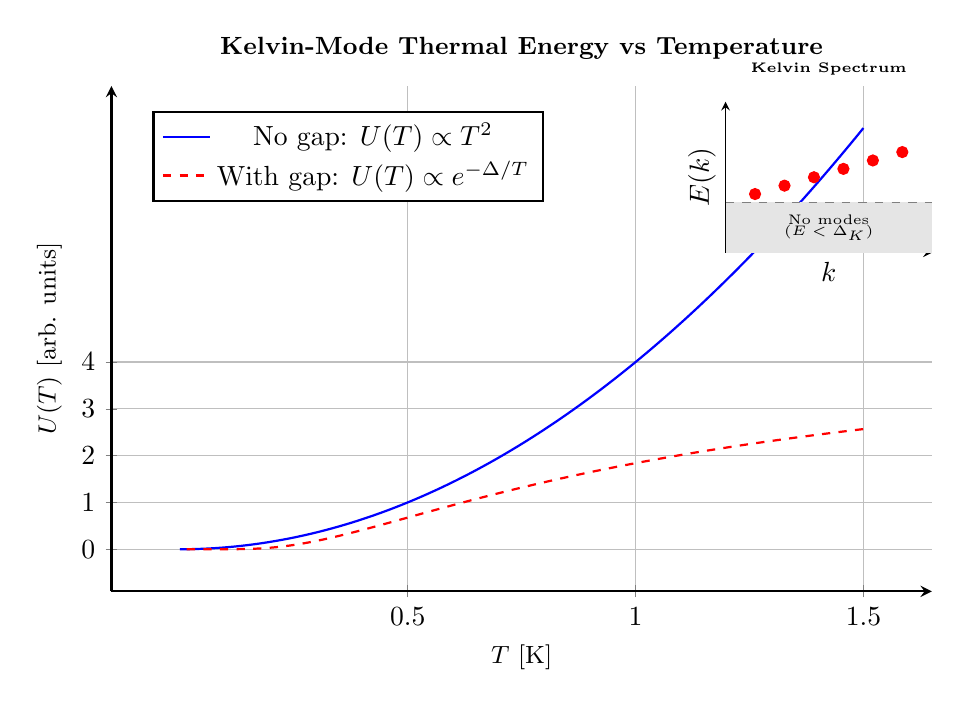
\begin{tikzpicture}
% MAIN PLOT: Thermal Energy vs Temperature
                \begin{axis}[
                width=12cm,
                height=8cm,
                xlabel={$T$ [K]},
                ylabel={$U(T)$ [arb. units]},
                legend style={at={(0.05,0.95)}, anchor=north west},
                domain=0:1.5,
                samples=100,
                axis lines=left,
                enlargelimits=true,
                grid=both,
                xtick={0.5,1.0,1.5},
                ytick={0,1,2,3,4},
                xlabel style={font=\small},
                ylabel style={font=\small},
                title={Kelvin-Mode Thermal Energy vs Temperature},
                title style={font=\bfseries\small},
                thick
                ]
% No Gap: U ~ T^2
                \addplot[blue,thick] {4*x^2};
                \addlegendentry{No gap: $U(T) \propto T^2$}
% With Gap: U ~ exp(-Δ/T)
                \addplot[red,thick,dashed] {5*exp(-1/x)};
                \addlegendentry{With gap: $U(T) \propto e^{-\Delta/T}$}
                \end{axis}

% INSET: Energy spectrum with gap
                \begin{scope}[shift={(7.8,4.3)}]
                    \begin{axis}[
                    width=4.2cm,
                    height=3.5cm,
                    title={Kelvin Spectrum},
                    title style={font=\bfseries\tiny},
                    xlabel={$k$},
                    ylabel={$E(k)$},
                    axis lines=left,
                    ticks=none,
                    xmin=0, xmax=3.5,
                    ymin=0, ymax=4.5,
                    xtick=\empty,
                    ytick=\empty,
                    clip=false
                    ]
                    \fill[gray!20] (axis cs:0,0) rectangle (axis cs:3.5,1.5);
                    \draw[dashed, gray] (axis cs:0,1.5) -- (axis cs:3.5,1.5);
                    \foreach \x in {0.5,1.0,1.5,2.0,2.5,3.0} {
                        \addplot[only marks, mark=*, red] coordinates {(\x, {1.5 + 0.5*\x})};
                    }
                    \node[align=center,font=\tiny] at (axis cs:1.75,0.75) {No modes\\[-0.3em]($E<\Delta_K$)};
                    \end{axis}
                \end{scope}
            \end{tikzpicture}
            \caption{Comparison of Kelvin-mode thermal energy with and without a topological excitation gap $\Delta_K$. Inset: discrete spectrum with a forbidden band $E<\Delta_K$.}
            \label{fig:kelvin-gap}
        \end{figure}

        \begin{figure}[htbp]
            \centering
            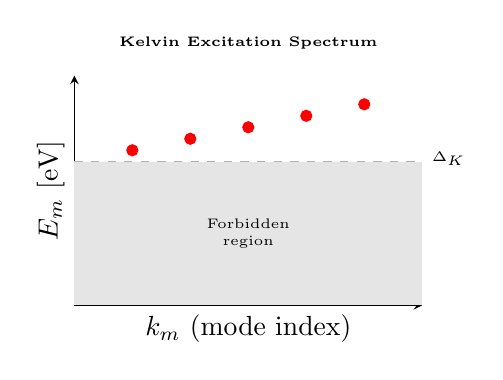
\begin{tikzpicture}
                \begin{axis}[
                width=6cm,
                height=4.5cm,
                title={Kelvin Excitation Spectrum},
                title style={font=\bfseries\tiny},
                xlabel={$k_m$ (mode index)},
                ylabel={$E_m$ [eV]},
                axis lines=left,
                ticks=none,
                xmin=0, xmax=6,
                ymin=0, ymax=800,
                clip=false
                ]
                \pgfmathsetmacro{\DeltaK}{500} % eV gap
                \fill[gray!20] (axis cs:0,0) rectangle (axis cs:6,\DeltaK);
                \draw[dashed, gray!60] (axis cs:0,\DeltaK) -- (axis cs:6,\DeltaK);
                \node[align=center,font=\tiny] at (axis cs:3,250) {Forbidden\\ region};
                \foreach \x in {1,2,3,4,5} {
                    \addplot[only marks, mark=*, red, mark size=2pt] coordinates {(\x, {\DeltaK + 40*\x})};
                }
                \node[anchor=west,font=\tiny] at (axis cs:6,\DeltaK+10) {$\Delta_K$};
                \end{axis}
            \end{tikzpicture}
            \caption{Illustrative Kelvin excitation spectrum with a gap $\Delta_K=\SI{500}{\electronvolt}$. Shaded band: $E<\Delta_K$.}
            \label{fig:kelvin-thermal-suppression}
        \end{figure}

        For finitely many Kelvin modes,
        \begin{equation}
            U_K^{(n)}(T) \lesssim N_K \Delta_K \exp\!\left(-\frac{\Delta_K}{k_B T}\right),
        \end{equation}
        replacing the dangerous polynomial scaling of the ungapped case.

        \begin{didactic}
            \emph{Takeaway.} With a gap, thermal activation is exponentially small: $U\sim e^{-\Delta_K/k_BT}$, not $\sim T^2$.
        \end{didactic}

% ============================================================
    \section{Required Gap Scale}\label{sec:required_gap}
        Imposing
        \begin{equation}
            a_n^{\mathrm{eff}} \lesssim 10^{-62}\,\si{J\,K^{-2}}
        \end{equation}
        yields
        \begin{equation}
            \frac{\Delta_K}{k_B T_{\mathrm{eff}}} \gtrsim 60.
        \end{equation}
        Using a conservative bound
        \begin{equation}
            T_{\mathrm{eff}} \lesssim 10^5\,\si{K},
        \end{equation}
        we obtain
        \begin{equation}
            \Delta_K \gtrsim 5\times 10^2\,\si{eV}.
        \end{equation}
        This sits far below $m_e c^2=\SI{511}{keV}$ yet far above atomic binding scales ($\sim\SI{10}{eV}$), so Kelvin modes are frozen in ordinary atomic physics.

        \begin{didactic}
            \emph{Numbers in context.} A few hundred eV is negligible compared to the electron’s rest energy but huge on atomic scales—exactly what we need for inert Kelvin modes.
        \end{didactic}

        Such a gap implies that Kelvin excitations remain frozen up to effective temperatures corresponding to electron accelerations of order $10^{22}\,\mathrm{m/s^2}$\textemdash far beyond terrestrial or typical laboratory regimes. Hence no measurable corrections to atomic spectra are expected under ordinary conditions, while high-acceleration or keV-MeV scattering experiments could in principle probe activation of these modes.

% ============================================================
    \section{Relation to the Schr\"odinger Equation}\label{sec:schrodinger}
        \begin{figure}[ht]
            \centering
            \includegraphics[width=0.85\textwidth]{hydro_energy_levels}
            \caption{\textbf{Hydrodynamic energy levels} for $n = 1,2,3,4$. The ground state ($n=1$) sets a laminar baseline; excited states scale approximately as $1/n^2$, matching the hydrogenic spectrum. These levels emerge from vortex equilibrium in an incompressible medium.}
            \label{fig:sst_hydrodynamic_levels}
        \end{figure}

        With Kelvin modes suppressed, a minimal free-energy functional is
        \begin{equation}
            \mathcal{F}[\psi]
            =
            \int d^3r\left[
                         \frac{\hbar^2}{2m_e} |\nabla\psi|^2 + V(r)\, |\psi|^2
            \right].
        \end{equation}
        Here $V(r)$ is taken as an \emph{effective} binding potential with far-field behavior
        $V(r)\sim -\Lambda/r$. In the corrected SST-consistent picture, a steady swirl with
        $v_\theta\propto 1/r$ yields a near-field pressure deficit $\Delta p\propto -1/r^2$ (Euler radial balance),
        while the far-field $1/r$ tail is modeled as Poisson-mediated (clock/foliation mediator on $\mathbb{R}^3$).
        Variation under normalization gives
        \begin{equation}
            -\frac{\hbar^2}{2m_e}\nabla^2\psi + V(r)\,\psi = E\,\psi,
        \end{equation}
        the stationary Schr\"odinger equation \cite{AbeOkuyama2011}.

        \begin{didactic}
            \emph{Bridge to QM.} In the Kelvin-frozen regime, hydrodynamics reproduces Schr\"odinger’s stationary equation as the Euler–Lagrange condition of $\mathcal{F}$.
        \end{didactic}

% ============================================================
    \section{Hydrodynamic Origin of the Schr\"odinger Equation}\label{sec:hydro_origin}
        Assuming a closed, knotted filament with internal excitations frozen, consider
        \begin{equation}
            \mathcal{F}[\psi]
            =
            \int d^3r\left[
                         \frac{\hbar^2}{2m_e}|\nabla\psi|^2 + V(r)\,|\psi|^2
            \right],\qquad \int |\psi|^2 d^3r = 1,
        \end{equation}
        with $V(r)$ an effective potential whose far-field asymptotic is $V(r)\sim -\Lambda/r$.
        The wording ``pressure potential'' is not meant as a claim that Euler pressure alone produces $1/r$;
        rather, the $1/r$ tail is attributed to a local mediator (Poisson/Green-function response), while
        Euler pressure motivates only the regularized core/near-field structure.
        Varying $\mathcal{F}$ yields
        \begin{equation}
            -\frac{\hbar^2}{2m_e}\nabla^2\psi + V(r)\,\psi = E\,\psi,
        \end{equation}
        i.e., the stationary Schr\"odinger equation.

        \begin{didactic}
            \emph{Same result, different route.} This re-derivation underlines that the reduction is robust to modeling details once Kelvin modes are inert.
        \end{didactic}

% ============================================================
    \section{Thermodynamic Catastrophe from Ungapped Kelvin Modes}\label{sec:catastrophe}
        If Kelvin modes couple thermodynamically to orbitals, one can parameterize
        \begin{equation}
            U_{\mathrm{Kelvin},n}(T_\ast)
            =
            a_n T_\ast^2 + \mathcal{O}(T_\ast^4),
            \qquad
            E_n^{\mathrm{eff}} = E_n^{(0)} - a_n T_\ast^2.
        \end{equation}
        A naive elastic estimate gives
        \begin{equation}
            a_n^{\text{naive}} \sim 10^{-39}\,\mathrm{J/K^2},
        \end{equation}
        while spectroscopy requires
        \begin{equation}
            a_n \lesssim 10^{-62}\,\mathrm{J/K^2}.
        \end{equation}
        The gap is therefore essential: without it, the $1/n^2$ spectrum collapses.

        \begin{didactic}
            \emph{Bottom line.} Ungapped Kelvin thermodynamics is a disaster for atoms; the gap prevents it.
        \end{didactic}

% ============================================================
    \section{Discussion and Outlook}\label{sec:outlook}
        A Kelvin excitation gap resolves a central consistency constraint in vortex-filament accounts of atomic structure. Atomic orbitals remain sharply quantized because Kelvin waves are exponentially suppressed at low energies, and the Schr\"odinger equation emerges as an effective equation of state in this Kelvin-frozen regime. This establishes a clean separation of scales: (1) low-energy, where hydrodynamic equilibrium reproduces quantum results; and (2) high-energy or high-acceleration domains, where Kelvin dynamics activate and new phenomenology may arise.

        This delivers a clear separation of scales:
        \begin{itemize}
            \item \textbf{Low energy}: Kelvin modes inert; orbital structure from hydrodynamic equilibrium, matching standard quantum results.
            \item \textbf{High energy / high acceleration}: Kelvin dynamics activate, enabling new phenomenology.
        \end{itemize}

        One possible Swirl-String framework (SST) realizes this broader picture by modeling electrons as topologically stable, knotted vortex filaments in a real, incompressible condensate. The present mainstream formulation dovetails with SST's claims: the same gapped Kelvin mechanism explains why low-energy atomic physics is effectively quantum-mechanical, while predicting activation of internal modes under extreme conditions.

        From an empirical perspective, possible signatures include slight broadening or phase lags in atomic transitions under extreme acceleration, and energy-loss features in high-field scattering consistent with Kelvin-mode activation thresholds near a few hundred eV. Quantum-clock and relativistic interferometry techniques \cite{SmithAhmadi2020,CastroRuiz2017} offer a future route to testing such coherence-dependent effects.

        Potentially relevant domains include:
        \begin{itemize}
            \item ultra-high accelerations (Unruh-like activation) \cite{Unruh1976},
            \item keV-MeV scattering,
            \item vortex reconnections in astrophysical or cosmological fluids.
        \end{itemize}

        More broadly, quantum-clock experiments access coherence-dependent time-dilation signatures \cite{SmithAhmadi2020,CastroRuiz2017}.
From a foundations standpoint, relational-time formalisms suggest treating clock observables as conditional dynamics within correlations.
 \cite{PageWootters1983,Wootters1984}.

        \begin{didactic}
            \emph{What to test.} Look for activation of Kelvin modes under extreme conditions; at ordinary atomic energies they should remain silent. SST provides one concrete framework where these effects can be modeled in detail.
        \end{didactic}

% ============================================================
        \appendix
    \section*{Appendix A: Estimate of First Kelvin Mode Energy}\label{app:first_kelvin}
        For the first mode ($m=1$) in the ground state ($n=1$), $L \sim 2\pi r_1 = 2\pi a_0 \approx \SI{3.3e-10}{m}$ with $a_0 \approx \SI{5.29e-11}{m}$. The circulation quantum $\Gamma=h/m_e$ gives $\Gamma \approx \SI{7.27e-4}{m^2/s}$.

        Then $k_1=2\pi/L \approx \SI{1.9e10}{m^{-1}}$ and
        \begin{equation}
            \omega_1 \simeq \frac{\Gamma}{4\pi} k_1^2 \!\left[ \ln\!\left( \frac{1}{k_1 \xi} \right) + C_0 \right],
        \end{equation}
        with $C_0\sim 1$ and $\xi \sim \SI{1e-15}{m}$, giving $\omega_1 \approx \SI{2.8e17}{rad/s}$ and
        \begin{equation}
            E_1=\hbar\omega_1 \approx \SI{29.5}{eV}.
        \end{equation}
        Tighter knots/smaller cores push this higher, consistent with a gap $\Delta_K \sim \SI{500}{eV}$.

% ============================================================
% Back matter (Springer Nature)
% ============================================================
        \backmatter
        \bmhead{Declarations}

        \subsection*{Funding}
            Not applicable.

        \subsection*{Competing interests}
            The author declares no competing interests.

        \subsection*{Ethics approval}
            Not applicable.

        \subsection*{Consent to participate}
            Not applicable.

        \subsection*{Consent for publication}
            Not applicable.

        \subsection*{Data availability}
            Not applicable.

        \subsection*{Materials availability}
            Not applicable.

        \subsection*{Code availability}
            Not applicable.

        \subsection*{Author contributions}
            O.I. conceived the study, developed the analysis, performed the derivations, and wrote the manuscript.

% ============================================================
% References
% ============================================================
            \begin{thebibliography}{99}

                \bibitem{Helmholtz1858}
                H.~Helmholtz,
                ``On Integrals of the Hydrodynamical Equations Which Express Vortex Motion,''
                \emph{J. Reine Angew. Math.} \textbf{55}, 25--55 (1858).

                \bibitem{Kelvin1867}
                W.~Thomson (Lord Kelvin),
                ``On Vortex Atoms,''
                \emph{Proc. R. Soc. Edinburgh} \textbf{6}, 94--105 (1867).

                \bibitem{Onsager1949}
                L.~Onsager,
                ``Statistical Hydrodynamics,''
                \emph{Nuovo Cimento Suppl.} \textbf{6}, 279--287 (1949).

                \bibitem{Feynman1955}
                R.~P.~Feynman,
                ``Application of Quantum Mechanics to Liquid Helium,''
                in \emph{Progress in Low Temperature Physics}, Vol.~1,
                North-Holland (1955).

                \bibitem{LordKelvin1880}
                W.~Thomson (Lord Kelvin),
                ``Vibrations of a Columnar Vortex,''
                \emph{Philosophical Magazine} \textbf{10}, 155--168 (1880).

                \bibitem{Barenghi2014}
                C.~F.~Barenghi, L.~Skrbek, and K.~R.~Sreenivasan,
                ``Introduction to Quantum Turbulence,''
                \emph{Proc. Natl. Acad. Sci. USA} \textbf{111}, 4647--4652 (2014).

                \bibitem{Ricca1996}
                R.~L.~Ricca,
                ``The Contributions of Da Rios and Levi-Civita to Asymptotic Potential Theory and Vortex Filament Dynamics,''
                \emph{Fluid Dynamics Research} \textbf{18}, 245--268 (1996).

                \bibitem{Pathria2011}
                R.~K.~Pathria and P.~D.~Beale,
                \emph{Statistical Mechanics}, 3rd ed.,
                Elsevier (2011).

                \bibitem{AbeOkuyama2011}
                S.~Abe and S.~Okuyama,
                ``Similarity between Quantum Mechanics and Thermodynamics,''
                \emph{Phys. Rev. E} \textbf{83}, 021121 (2011).

                \bibitem{Unruh1976}
                W.~G.~Unruh,
                ``Notes on Black-Hole Evaporation,''
                \emph{Phys. Rev. D} \textbf{14}, 870--892 (1976).

                \bibitem{Madelung1926}
                E.~Madelung,
                ``Quantentheorie in hydrodynamischer Form,''
                \emph{Z. Phys.} \textbf{40}, 322--326 (1926).

                \bibitem{Bohm1952}
                D.~Bohm,
                ``A Suggested Interpretation of the Quantum Theory in Terms of `Hidden' Variables. I.,''
                \emph{Phys. Rev.} \textbf{85}, 166--179 (1952).

                \bibitem{Couder2006}
                Y.~Couder, S.~Proti\`ere, E.~Fort, and A.~Boudaoud,
                ``Dynamical phenomena: Walking and orbiting droplets,''
                \emph{Nature} \textbf{437}, 208 (2005).

                \bibitem{PageWootters1983}
                D.~N.~Page and W.~K.~Wootters,
                \textit{Evolution without evolution: Dynamics described by stationary observables},
                Physical Review D \textbf{27} (1983) 2885.
                doi:10.1103/PhysRevD.27.2885

                \bibitem{Wootters1984}
                W.~K.~Wootters,
                \textit{``Time'' replaced by quantum correlations},
                International Journal of Theoretical Physics \textbf{23} (1984) 701--711.
                doi:10.1007/BF02214098

                \bibitem{SmithAhmadi2020}
                A.~R.~H.~Smith and M.~Ahmadi,
                \textit{Quantum clocks observe classical and quantum time dilation},
                Nature Communications \textbf{11} (2020) 5360.
                doi:10.1038/s41467-020-18264-4

                \bibitem{CastroRuiz2017}
                E.~Castro-Ruiz, F.~Giacomini, and \v{C}.~Brukner,
                \textit{Entanglement of quantum clocks through gravity},
                Proceedings of the National Academy of Sciences \textbf{114} (2017) E2303--E2309.
                doi:10.1073/pnas.1616427114

            \end{thebibliography}

\end{document}